%%%%%%%%%%%%%%%%%%%%%%%%%%%%%%%%%%%%%%%%%%%%%%%%%%%%
%%											  	 %%
%% Author : Andreas Apostolatos               	 %%
%%											  	 %%
%% e-mail : andreas.apostolatos@tum.de		   	 %%
%%											  	 %%
%% 02_Theoretical_background.tex				 %%
%%											  	 %%
%%%%%%%%%%%%%%%%%%%%%%%%%%%%%%%%%%%%%%%%%%%%%%%%%%%%

\section{Theoretical Background}
\subsection{What is a Sensitivity Analysis?}
In general, a sensitivity analysis is a study on how output variables change according to a modification of the input parameter. In the field of structural analysis, it is used to determine the gradient of a response function which are used as objective or constraint. \\[6pt]
In the design process, this naturally leads to optimization: through a modification of the input data, an influence on the performance of the structure can be observed. \\[6pt]
In this report, a response sensitivity analysis will be taken into account.\\

\subsection{Response sensitivity analysis}
In general, optimal designs are characterized by the \textit{Karush-Kuhn-Tucker} condition, which states
\begin{equation}
\dv{L}{\textbf{x}} = \dv{f}{\textbf{x}} + \lambda^T  \dv{\textbf{g}}{\textbf{x}} 
%Lambda should be Bold
\end{equation}
where $f$ represents the objective function, $\textbf{g}$ the constraints and $\textbf{x}$ the optimization variables.
In general, structural response functions $f$ and $g$ depend on the design variables $\textbf{x}$ as well as the response variables $\textbf{u}$ which are usually represented by the structural displacements. \\
In mathematical terms, this is represented by the following relationships: 
\begin{equation}
f = f \big(\textbf{u}, \textbf{u(x)}\big)
\end{equation}
According to the chain rule, the differentiation of the objective function with respect to the design variables is
\begin{equation}
\dv{f}{\textbf{x}} = \pdv{f}{\textbf{x}} + \pdv{f}{\textbf{u}} \dv{\textbf{u}}{\textbf{x}}
\end{equation}

\subsection{Sensitivity of the response variables}
As said, in response sensitivity analysis the response variables \textbf{u} are represented by the nodal displacements; and the main task is to find the derivative of \textbf{u} with respect to the design variables \textbf{x}.\\Considering a typical displacement formulation of the finite elements method, the equilibrium condition is represented by 
\begin{equation}
\textbf{K}\textbf{u} = \textbf{P}
\end{equation}
where 
\begin{itemize}
\item \textbf{K}: system stiffness matrix 
\item \textbf{u}: vector of nodal displacements
\item \textbf{P}: load vector
\end{itemize}
Derivation with respect to \textbf{x} yields 
\begin{equation}
\dv{(\textbf{K}\textbf{u})}{\textbf{x}} = \dv{\textbf{P}}{\textbf{x}}
\end{equation}
\begin{equation}
\dv{\textbf{K}}{x}\textbf{u} + \textbf{K} \dv{\textbf{u}}{\textbf{x}} = \dv{\textbf{P}}{\textbf{x}}
\end{equation}
\begin{equation}
\dv{\textbf{u}}{\textbf{x}} = \textbf{K}^{-1} \Big(\dv{\textbf{P}}{\textbf{x}} - \dv{\textbf{K}}{\textbf{x}} \textbf{u}\Big)
\end{equation}
The right end side of (7-last) is called \textit{pseudo force vector} $\textbf{P}^{\ast}$ \cite{optimization_Bletzinger}.

\subsection{Analytical method}
First of all, a direct approach is taken into account. This means that, in order to approximate the derivative of a response function, $g_j(\textbf{x}, \textbf{u}(\textbf{x}))$ with respect to $x_i$, i.e.:
\begin{equation} \label{eqn:responsefctderivative}
\dv{g_j}{x_i} = \pdv{g_j}{x_i} + \pdv{g_j}{\textbf{u}} \pdv{\textbf{u}}{x_i} = \pdv{g_j}{x_i} + \pdv{g_j}{\textbf{u}} \textbf{K}^{-1} (\dv{\textbf{P}}{x_i} - \dv{\textbf{K}}{x_i}\textbf{u})
%Cambiare parentesi
%\label{2.1}
\end{equation}
which means that, through a direct approach, 
\begin {itemize}
\item first, $\dv{\textbf{u}}{x_i}$ is computed by solving $\textbf{K}^{-1}\textbf{P}_i^{\ast}$;
\item then, $\dv{\textbf{u}}{x_i}$ is substituted into (2.1) and $\textbf{K}^{-1}\textbf{P}_i^{\ast}$ needs to be solved $n$ times, where $n$ represents the number of design variables. \cite{optimization_Bletzinger}
\end{itemize}

\subsection{Adjoint method}
Otherwise, the operation order can be reversed. The starting point, as illustrated before, is still the following: 
\begin{equation}
\dv{g_j}{x_i} = \pdv{g_j}{x_i} + \pdv{g_j}{\textbf{u}} \pdv{\textbf{u}}{x_i} =\textbf{K}^{-1} (\dv{\textbf{P}}{x_i} - \dv{\textbf{K}}{x_i}\textbf{u})
%Cambiare parentesi
%\label{2.1}
\end{equation}
First of all, the \textit{adjoint variables} $\widetilde{\textbf{u}}_j$ can be calculated as 
\begin{equation} \label{eqn:adjointVariable}
\widetilde{\textbf{u}}_j = \textbf{K}^{-1} \pdv{g_j}{\textbf{u}}
\end{equation}
and the results can be later inserted in the remaining formula. \\[3pt]
Equation \ref{eqn:adjointVariable} above has to be solved $m$ times, where $m$ represents the number of response functions $g_j$ \cite{optimization_Bletzinger}.

\subsection{Finite difference approximation}
The complexity of the element formulation makes the sensitivity analysis very hard, sometimes impossible to code. For this reason, a finite element approximation is used most of the times. \\[6pt]
The first order derivative of a function $f$ with respect to $x_i$ can be approximated by the formula 
\begin{equation}
\pdv{f}{x_i} \cong \frac{f(x_i + \Delta x_i) - f(x_i)}{\Delta x_i}
\end{equation}
Since a complete analytical resolution of the system would be heavily time consuming, semi-analytical approaches are taken into account. This means that a mixture of both analytical and numerical methods is considered: equations are developed analytically, then all derivatives are replaced by their numerical approximation.
In this case, no additional element code is needed. \cite{optimization_Bletzinger}
\subsubsection{Differencing schemes}
In the script, several differencing schemes are taken into account. 
In this section, a quick look at the possible different ones is taken. Three methods exist to approximate the derivative of a function, \textit{forward}, \textit{backward} and \textit{central} differencing.\\[6pt]
Considering the formula 
\begin{equation}
\pdv{f}{x_i} \cong \frac{f(x_i + \Delta x_i) - f(x_i)}{\Delta x_i}
\end{equation}
%Inserire fonte immagine
\begin{figure}[ht]
  \centering
  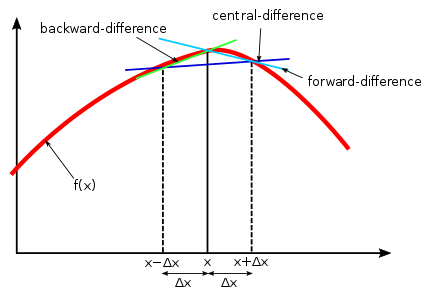
\includegraphics[width=110mm]{images/differencing.png}
  \caption{Visual illustration of differencing schemes\\ \cite{wiki:finiteDifference}}
  \label{fig:differencingschemes}
\end{figure}
In Figure \ref{fig:differencingschemes}, a visual representation of the differences between the approximation schemes is shown on a generic function taken as an example.
It is possible to see how the result of the approximation depends on the choice of $\Delta x_i$.
In particular, a step in the positive or negative direction can be taken, as well as in both of those. Respectively, these choices lead to forward, backward and central differencing method. \cite{masching_dissertation} \\[6pt]
Later on, it will be explained how the choice of the differencing scheme affects the results of the analysis.





